% ===== UNIT 23: Ablation study (5.4) =====
% Status: REWRITTEN  (change to REWRITTEN / REVIEWED when done; see CHECKLIST.md)
% Rules: style rewrite only. Keep every \cite, \ref, \label, number, equation and table value as is. Change the wording, not the content.
\subsection{Ablation study}
Table~\ref{tab:ablation} traces the complete performance trajectory. Figures~\ref{fig:trajectory} and~\ref{fig:isolated} show it visually. The endpoint values are verified against published results~\cite{he2021transreid} and repository experiment logs. All intermediate rows are measured from isolated ablation experiments.

\begin{table*}[!t]
  \centering
  \caption{Stepwise ablation: 82.3\% $\to$ 93.3\% mAP on VeRi-776.
    Rows A1--A5$\beta$ report isolated-component contributions measured under a
    common operating point (Stream~1 only, AQE $k{=}3$ $+$ $k$-reciprocal
    re-ranking, single-flip 768D CLS). Deltas are relative to control A1.
    \textbf{A1 is an intentionally minimal, un-tuned SGD control}
    (ImageNet-initialised DeiT, no recipe or schedule tuning). It is not a
    reproduction of TransReID, whose fully tuned DeiT-B SGD recipe reaches
    82.3\% mAP~\cite{he2021transreid}. The isolated deltas show component
    contributions during recipe development relative to this control. They
    must not be read as head-to-head superiority over a tuned baseline. The
    cumulative trajectory (lower block) is the authoritative
    recipe-versus-published accounting, anchored at the published 82.3\%%
    \protect\footnotemark}
  \label{tab:ablation}
  \small
  \begin{tabular}{L{8.6cm}C{1.6cm}C{1.6cm}C{1.8cm}}
    \toprule
    Configuration & mAP~(\%) & R1~(\%) & $\Delta$ vs.\ A1 \\
    \midrule
    \multicolumn{4}{l}{\emph{Isolated component ablation (Stream~1, AQE $+$ rerank)}} \\
    A1, un-tuned SGD control (DeiT $+$ SGD $+$ CE $+$ triplet, not TransReID) & 57.62 & 80.45 & -- \\\\
    A2, $+$CLIP initialisation only                    & 70.97 & 86.83 & $+13.35$ \\
    A3, $+$SupCon only (DeiT $+$ SGD $+$ CE-LS $+$ SupCon) & 59.48 & 79.74 & $+1.86$ \\
    A4, $+$AdamW/LLRD only (DeiT $+$ CE $+$ triplet)   & 80.91 & 94.82 & $+23.29$ \\
    A5$\alpha$, full (CLIP $+$ AdamW/LLRD $=0.75$ $+$ CE-LS $+$ triplet $+$ centre, deployed) & 89.06 & 97.74 & $+31.44$ \\
    A5$\beta$, full (CLIP $+$ AdamW/LLRD $=0.65$ $+$ CE-LS $+$ SupCon, alternative) & 88.57 & 96.66 & $+30.95$ \\
    \midrule
    \multicolumn{4}{l}{\emph{Cumulative trajectory $\to$ headline}} \\
    TransReID baseline (DeiT-B*)~\cite{he2021transreid}  & 82.30 & 97.10 & -- \\\\
    Base cosine, ViT-B (no PP)                            & 82.22 & 97.50 & $-0.08$ \\
    \quad$+$AQE $k{=}3$                                   & 84.08 & 97.20 & $+1.86$ \\
    \quad$+$rerank $k_1{=}80,k_2{=}15,\lambda{=}0.2$      & 89.63 & 97.74 & $+5.55$ \\
    \quad$+$concat-patch $+$ flip TTA (1536D, A5$\alpha$, deployed) & 89.97 & 97.79 & $+0.34$ \\
    \midrule
    CLIP-SENet v6, base cosine~\cite{lu2025clipsenet}     & 82.34 & 96.54 & -- \\\\
    \quad$+$AQE $k{=}10$                                  & 89.21 & 96.90 & $+6.87$ \\
    \quad$+$rerank $k_1{=}50,k_2{=}10,\lambda{=}0.1$      & 91.44 & 97.08 & $+2.23$ \\
    \midrule
    \textbf{Fusion ($w_1{=}0.35$, $w_2{=}0.65$)}          & \textbf{93.32} & \textbf{98.45} & $+1.88$ \\
    \bottomrule
  \end{tabular}
\end{table*}

\footnotetext{The cumulative-trajectory rows are the deterministic evaluation of frozen, SHA-256-pinned checkpoints. The isolated-ablation rows (A1--A5$\beta$) are single from-scratch training runs. Only the deployed A5$\alpha$ recipe was characterised for seed variance ($\pm 0.55$\,pp, Section~\ref{sec:seed_variance}). The isolated controls A1--A4 were not individually seed-repeated, so their absolute values carry at least this much training noise. See Section~\ref{sec:reproducibility} for checkpoint hashes and the two reproducibility regimes.}

\begin{figure*}[!t]
  \centering
  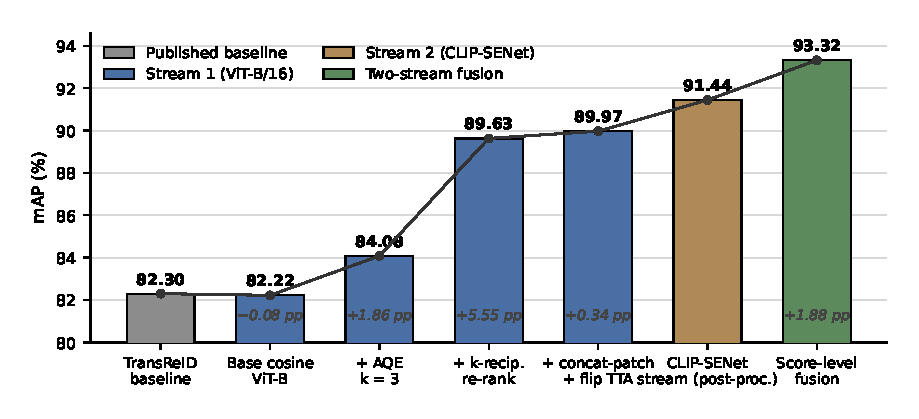
\includegraphics[width=\textwidth]{Fig5}
  \caption{Cumulative performance trajectory on VeRi-776 from the published
  TransReID baseline to the two-stream fusion, under a single consistent
  post-processing protocol. The largest single step is $k$-reciprocal
  re-ranking on Stream~1 ($+5.55$\,pp). The recipe itself adds
  essentially nothing at the raw-embedding level ($-0.08$\,pp against the
  published baseline)}
  \label{fig:trajectory}
\end{figure*}

\begin{figure}[!t]
  \centering
  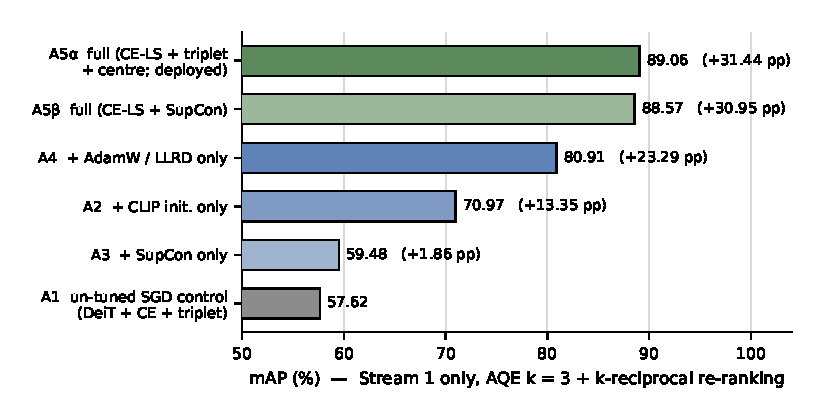
\includegraphics[width=\columnwidth]{Fig6}
  \caption{Isolated component ablation for the Stream~1 recipe, measured
  against the un-tuned SGD control A1 at a common operating point. The deltas
  quantify component contributions during recipe development and must not be
  read as head-to-head superiority over a tuned baseline, since A1 is
  deliberately un-tuned}
  \label{fig:isolated}
\end{figure}

The isolated-component block shows which ingredients our recipe depends on, relative to the un-tuned A1 control. AdamW with layer-wise LR decay (A4) gives the largest change, $+23.29$\,pp over the un-tuned SGD control A1. CLIP initialisation (A2) is next at $+13.35$\,pp. The A4 delta mostly reflects how hard it is to tune SGD under our short schedule. It does not mean that AdamW is $+23$\,pp better than SGD, because a fully tuned SGD recipe (TransReID) already reaches 82.3\% mAP~\cite{he2021transreid}. What A4 shows is that AdamW with layer-wise LR decay reaches a strong operating point without special schedule tuning for each optimiser. The recipe relies on this property in practice. SupCon alone (A3) barely helps ($+1.86$\,pp). But it combines well once CLIP and AdamW are in place. The deployed A5$\alpha$ recipe reaches 89.06\% mAP, which is statistically indistinguishable from the alternative A5$\beta$ recipe (88.57\% mAP). The difference is 0.49\,pp in a single run, which is within the $\pm 0.55$\,pp three-seed standard deviation of A5$\alpha$ (88.75\,$\pm$\,0.55\,pp, see Section~\ref{sec:seed_variance}). In the cumulative trajectory, the most important post-processing step is $k$-reciprocal re-ranking~\cite{zhong2017rerank} on Stream~1 ($+5.55$\,pp). AQE~\cite{arandjelovic2012aqe} adds $+1.86$\,pp, and TTA adds $+0.34$\,pp. Fusion gives $+1.88$\,pp above the stronger post-processed CLIP-SENet stream. This confirms that the two feature spaces complement each other.
